\section{Partial Identification via Optimal Transport}  \label{sec:pid}


\subsection{CCOT Formulation of Partial Identification}\label{subsec:ot_formulation}
In this section, we demonstrate how to derive tight, closed-form bounds for the PRTE. We begin by formally mapping the partial identification problem into an optimal transport framework.

The core intuition is to search over all possible joint distributions of the latent and observable variables $(Y(0), Y(1), U, X, Z, W)$ that are compatible with both the observed data and the structural conditions in \cref{asp:structure}. Because the potential outcomes are conditionally independent of the instrument given $X$, the identifying power of our model is entirely captured by the joint distributions of $(Y(w), U, X)$ for $w \in \{0, 1\}$.

Let $\pi_w$ denote the joint probability measure of $(Y(w), U, X)$ and let $\pi_w(\cdot\mid x,u)$ denote the conditional distribution of $Y(w)$ given $x,u$. Recall that our target parameter is a linear functional of these measures:
\[\theta_\omega(\pi_0, \pi_1) = \mathbb{E}_{(X,U,Y(1))\sim\pi_1} [Y(1) \omega(X,U)] - \mathbb{E}_{(X,U,Y(0))\sim\pi_0} [Y(0) \omega(X,U)]. \]
To achieve sharp bounds, we must constrain $\pi_w$ using all available observational information. Let $\mathbb{P}_{obs}$ denote the true observed joint distribution of $(Y, W, Z, X)$. Under the threshold-crossing model in \cref{asp:structure}, while $U$ is generally unobserved, its conditional distribution is explicitly tied to the treatment status and the propensity score. Specifically, conditional on $X$ and $Z$, the event $W=1$ perfectly corresponds to $U \leqslant p(Z,X)$, and $W=0$ corresponds to $U > p(Z,X)$.

\noindent\textit{Remark (notation).} For $w\in\{0,1\}$, $\pi_w$ denotes a joint probability law of $(Y(w),U,X)$, including a candidate such law when varied in the CCOT program, and $\pi_w(\cdot\mid u,x)$ denotes a measurable regular conditional outcome law determined only $\pi_w$-almost everywhere with respect to its $(U,X)$-marginal.


Together with the observed distribution of $(X,Z)$, the joint distributions $\pi_0$ and $\pi_1$ fully determine the observational distribution of $(X,Z,W,Y)$. To see this, we can link the unknown structural distributions directly to the observed conditional distribution of the data by exploiting the consistency equation $Y = W Y(1) + (1-W) Y(0)$ and the selection mechanism $W = \indicator(U \leqslant p(Z,X))$. For any measurable set $A \subseteq \mathcal{Y}$, the following identity holds for $\mathbb P_{Z,X}$-almost every $(z,x)$:
\begin{align*}
    \mathbb{P}_{obs}(Y \in A, W=1 \mid Z=z, X=x) &= \mathbb{P}(Y(1) \in A, U \leqslant p(z,x) \mid Z=z, X=x).
\end{align*}
By the conditional independence assumption $Z \indep (Y(1), U) \mid X$, we can omit $Z$ in the second conditioning:
\begin{align*}
    \mathbb{P}(Y(1) \in A, U \leqslant p(z,x) \mid Z=z, X=x) &= \mathbb{P}(Y(1) \in A, U \leqslant p(z,x) \mid X=x).
\end{align*}
Since instruments that generate the same propensity value $p(z,x)$ yield the same right-hand side conditional on $X=x$, we can replace conditioning on the full instrument value $Z=z$ with conditioning on the scalar propensity value $p(Z,X)=p(z,x)$ together with $X=x$. Next, we disintegrate the joint measures $\pi_w$ into the conditional distribution of the potential outcome given the covariates and the latent variable. The threshold-crossing rule selects $U \leqslant p(z,x)$ into treatment and $U > p(z,x)$ out of it, so write $\mathcal{R}_1(p) \coloneqq (0,p]$ and $\mathcal{R}_0(p) \coloneqq (p,1]$ for the two selected regions. Because $U \mid X \sim \text{Unif}(0,1)$, integrating over $\mathcal{R}_w(p)$ yields, for $P\mid X=x$-almost every $p$ and each $w \in \{0,1\}$,
\begin{align*}
    \mathbb{P}_{obs}(Y \in A, W=w \mid p(Z,X)=p, X=x) &= \int_{\mathcal{R}_w(p)} \pi_w(A \mid u, x) \,\mathrm{d}u.
\end{align*}
Write $P=p(Z,X)$. Because a regular conditional law at an exact value of a continuous propensity score is defined only almost surely, first define, for $P\mid X=x$-almost every $p$, the observed finite-measure-valued maps
\begin{equation}\label{eq:canonical_submeasures}
    H_{w,x}(p,\mathrm{d}y)\coloneqq
    \mathbb P_{\mathrm{obs}}(Y\in\mathrm{d}y,W=w\mid P=p,X=x),
    \qquad w\in\{0,1\}.
\end{equation}
To select canonical versions at every point of the conditional propensity support, let $K_{w,x}(\mathrm{d}y\mid u)$ be a regular conditional law of $Y(w)$ given $(U,X)=(u,x)$. Under \cref{asp:structure}, the preceding derivation gives
\[
    H_{w,x}(p,\mathrm{d}y)=\int_{\mathcal{R}_w(p)} K_{w,x}(\mathrm{d}y\mid u)\,\mathrm{d}u,
    \qquad w\in\{0,1\},
\]
for $P\mid X=x$-almost every $p$. The right-hand sides are Lipschitz in total variation and hence extend the observed equivalence classes in~(\ref{eq:canonical_submeasures}) continuously to $\operatorname{supp}(P\mid X=x)$. This extension is unique: two continuous versions that agree almost surely under the conditional law of $P$ agree everywhere on its support. We henceforth use $H_{w,x}$ for these canonical observed versions. Thus $H_{w,x}$ is identified from $\mathbb P_{\mathrm{obs}}$ on the conditional propensity support, including its endpoints even when the corresponding singleton events have probability zero; the latent kernels $K_{w,x}$ themselves need not be identified. With no covariates we write $H_w$.
Furthermore, by construction, the marginal distribution of $(U, X)$ under $\pi_w$ must equal the known population distribution $\mathbb{P}_{U,X}$.

\noindent\textit{Remark (notation).} $P=p(Z,X)$ is the observed baseline propensity index obtained by evaluating the population propensity function at $(Z,X)$. In Proposition~\ref{prop:continuous_reduction}, Theorem~\ref{thm:continuous_rate}, Corollary~\ref{cor:continuous_primitive_rate}: The conditional propensity support is $\operatorname{supp}(P\mid X=x)=[\underline p(x),\overline p(x)]$ in the connected-instrument setting. In Theorem~\ref{thm:discrete_lower_bound}, Theorem~\ref{thm:continuous_lower_bound}: With $X$ almost surely constant, the covariate argument is suppressed and $P=p(Z)$. $\mathcal R_w$ is the selected-region map for $w\in\{0,1\}$ and $p\in[0,1]$, with $\mathcal R_1(p)=(0,p]$ and $\mathcal R_0(p)=(p,1]$, including empty intervals at the corresponding boundary propensities. For $w\in\{0,1\}$ and almost every $x$, $H_{w,x}$ is the unique total-variation-continuous version on $\operatorname{supp}(P\mid X=x)$ of $\mathbb P_{\mathrm{obs}}(Y\in\mathrm dy,W=w\mid P=p,X=x)$, including support endpoints; its total mass is $p$ for $w=1$ and $1-p$ for $w=0$, and without covariates it is written $H_w$. $H_w$, $w\in\{0,1\}$, denotes the no-covariate canonical continuous version of $\mathbb P_{\mathrm{obs}}(Y\in\mathrm{d}y,W=w\mid P=p)$ on $\operatorname{supp}(P)$, uniquely determined there by its almost-sure observed values. In Theorem~\ref{thm:continuous_lower_bound}: $H_1(0,\cdot)=0$ is specified even when $0$ lies outside propensity support, so the initial gap uses a structural boundary submeasure. $K_{w,x}(\mathrm dy\mid u)$, for $w\in\{0,1\}$, is a regular conditional probability kernel for $Y(w)$ given $(U,X)=(u,x)$ under a compatible latent law, determined only $\mathbb P_{U,X}$-almost everywhere and not necessarily identified, with $H_{w,x}(p,\mathrm dy)=\int_{\mathcal R_w(p)}K_{w,x}(\mathrm dy\mid u)\,\mathrm du$ on the conditional propensity support for $\mathbb P_X$-almost every $x$.


This allows us to formulate the partial identification of the PRTE as the following infinite-dimensional linear programming problem, in which every constraint is imposed for both $w \in \{0,1\}$:
\begin{equation}\label{eq:ot_formulation}
    \begin{split}
        \max_{\pi_0, \pi_1} \ / \min_{\pi_0, \pi_1}\quad & \theta_\omega(\pi_0, \pi_1)\\
        \text{subject to}  \quad &  \int_{\mathcal{R}_w(p(z,x))} \pi_w(\mathrm{d}y \mid u, x) \mathrm{d}u = H_{w,x}(p(z,x),\mathrm{d}y), \quad \mathbb P_{Z,X}\text{-a.e. }(z,x),\\
        & \pi_w(\mathrm{d}x, \mathrm{d}u) = \mathrm{d}u \ \mathbb{P}_{obs}(\mathrm{d}x),\\
        & \pi_w \text{ is supported on } \mathcal{Y} \times [0,1] \times \mathcal{X}.
    \end{split}
\end{equation}
We call the optimization in (\ref{eq:ot_formulation}) the Constrained Conditional Optimal Transport (CCOT) problem. The feasible set is constrained by the observational compatibility conditions in (\ref{eq:ot_formulation}); the problem is conditional in that, for fixed covariates $x$ and latent resistance $u$, it seeks a conditional measure $\pi_w(\cdot \mid u, x)$ on $\mathcal{Y}$; and it is a transport problem because the objective is linear in $\pi_w(\cdot \mid u, x)$ with effective cost $c(y, u, x) = y \cdot \omega(x, u)$, so that mass is transported from the latent space $U$ to the outcome space $Y(w)$ conditional on $X$.

To formally guarantee that the CCOT formulation in (\ref{eq:ot_formulation}) yields sharp bounds for the PRTE, we must show that any pair of measures $(\pi_0, \pi_1)$ satisfying the CCOT constraints corresponds to a valid data-generating process that satisfies our structural assumptions and perfectly reproduces the observed data. Let $\Gamma(\mathbb{P}_{obs})$ be the set of all measure pairs $(\pi_0, \pi_1)$ satisfying the constraints in (\ref{eq:ot_formulation}). The following proposition characterizes the joint distribution of $(Y(0), Y(1), U, X)$, from which observational
equivalence of the marginal pair $(\pi_0, \pi_1)$ follows immediately.

\begin{proposition}[Sharp Identified Set of the Joint Latent Law] \label{prop:sharpness}
    Suppose the observed distribution $\mathbb{P}_{obs}$ is generated by a true structural model satisfying \cref{asp:structure}. Let $\tilde{\pi}$ be any probability measure on $\mathcal{Y} \times \mathcal{Y} \times [0,1] \times \mathcal{X}$ whose $(Y(w), U, X)$-marginals $\tilde{\pi}_w$ satisfy $(\tilde{\pi}_0, \tilde{\pi}_1) \in \Gamma(\mathbb{P}_{obs})$. Then there exists a joint distribution of the latent and observable variables $(Y(0), Y(1), U, X, Z, W)$ such that:
    \begin{enumerate}
        \item[(i)] the joint marginal distribution of $(Y(0), Y(1), U, X)$ is exactly $\tilde{\pi}$;
        \item[(ii)] \cref{asp:structure} holds for $(Y(0), Y(1), U, X, Z, W)$;
        \item[(iii)] the induced distribution of $(Z, X, W, Y)$ exactly matches $\mathbb{P}_{obs}$.
    \end{enumerate}
    Conversely, every joint marginal $\tilde{\pi}$ arising from a distribution of $(Y(0), Y(1), U, X, Z, W)$ satisfying \textup{(ii)}--\textup{(iii)} has $(Y(w), U, X)$-marginals in $\Gamma(\mathbb{P}_{obs})$ for $w \in \{0, 1\}$.
\end{proposition}

\noindent\textit{Remark.} Every constraint in $\eqref{eq:ot_formulation}$ is imposed simultaneously for both $w\in\{0,1\}$.

\noindent\textit{Remark (notation).} $\tilde{\pi}$ is a probability measure on $\mathcal Y^2\times[0,1]\times\mathcal X$, interpreted as a candidate joint law of $(Y(0),Y(1),U,X)$. In Proposition~\ref{prop:sharpness}: Its marginals satisfy $(\tilde{\pi}_0,\tilde{\pi}_1)\in\Gamma(\mathbb P_{obs})$, hence its $(U,X)$-marginal is $\mathrm du\,\mathbb P_{obs}(\mathrm dx)$; the coupling of $Y(0)$ and $Y(1)$ conditional on $(U,X)$ is unrestricted apart from those marginal constraints. For $w\in\{0,1\}$, $\tilde{\pi}_w$ is the $(Y(w),U,X)$-marginal of $\tilde{\pi}$. In Proposition~\ref{prop:sharpness}: The pair satisfies $(\tilde{\pi}_0,\tilde{\pi}_1)\in\Gamma(\mathbb P_{obs})$, so $\tilde{\pi}_w(\mathrm du,\mathrm dx)=\mathrm du\,\mathbb P_{obs}(\mathrm dx)$ and its conditional outcome kernels satisfy the observational constraints in (\ref{eq:ot_formulation}); these kernels are defined up to $(\mathrm du\otimes\mathbb P_{obs}(\mathrm dx))$-null sets.


The content of \cref{prop:sharpness} is twofold. First, the CCOT constraints act only on the two marginals $\tilde{\pi}_0$ and $\tilde{\pi}_1$: any coupling of these marginals---including every joint law of $(Y(0), Y(1))$ given $(U, X)$---is observationally equivalent. Second, the converse makes the characterization sharp: no joint law outside this set can be generated by a structural model matching $\mathbb{P}_{obs}$. Consequently, the identified set for the PRTE target is $\{\theta_\omega(\pi_0, \pi_1) : (\pi_0, \pi_1) \in \Gamma(\mathbb{P}_{obs})\}$, and the maximum and minimum of $\theta_\omega(\pi_0, \pi_1)$ over $\Gamma(\mathbb{P}_{obs})$ are the sharp upper and lower bounds on the PRTE. The proof is given in \cref{app:proofs_pid}.

\begin{remark}
The fact that the moment relaxation approach of \citet{magne2018using} can yield arbitrarily loose bounds compared to our CCOT formulation is well-recognized; see also \citet{han_yang2024computational}. A detailed comparison example is given in \cref{exp:loose_bd} of \oalocation.
\end{remark}

\begin{remark}[Beyond PRTE: CCOT for general joint functionals]\label{rem:general_functional}
The CCOT perspective is not specific to the PRTE. At a conceptual level, one could consider a bounded measurable cost $f:\mathcal{Y}^2 \to \mathbb{R}$ and the joint target $\theta_f := \mathbb{E}[f(Y(1),Y(0))]$ by replacing the PRTE objective in (\ref{eq:ot_formulation}) with $\mathbb{E}_{\pi}[f(Y(1),Y(0))]$ and enlarging the decision variable from the pair $(\pi_0,\pi_1)$ to a joint conditional kernel $\pi(\diff y_1,\diff y_0 \mid u,x)$ whose marginals satisfy the same observational constraints. A sharp characterization should again follow from the lifting logic behind \cref{prop:sharpness}. What is special about the PRTE is the separable product cost $y \cdot \omega(x,u)$: it allows the CCOT problem to collapse into one-dimensional OT problems for each potential outcome separately. For a general joint functional, that separability is lost, and the resulting interval-specific problems are instead OT problems over the coupling between the identified marginals of $Y(1)$ and $Y(0)$, with no comparable closed-form reduction in general. Since the present paper is about the PRTE case, we do not pursue this extension here.
\end{remark}



Next, we show how to obtain a closed-form solution to the CCOT problem (\ref{eq:ot_formulation}).
Notice that in (\ref{eq:ot_formulation}), the objective is the difference of two linear functionals of $\pi_0$ and $\pi_1$, and the constraints on $\pi_0$ and $\pi_1$ are separate. Therefore, we only need to consider one side of the problem, as the other side follows identically. In what follows, we only consider the $W=1$ side minimization problem, i.e., 
\begin{equation}\label{eq:ot_formulation_1}
    \begin{split}
    \min_{ \pi_1}\quad &  \mathbb{E}_{\pi_1}[Y(1)\omega(X,U)]\\
        \text{subject to}  \quad &  \int_0^{p(z,x)} \pi_1(\mathrm{d}y \mid u, x) \mathrm{d}u = H_{1,x}(p(z,x),\mathrm{d}y),\quad \mathbb P_{Z,X}\text{-a.e. }(z,x)\\ 
        & \pi_1(\mathrm{d}x, \mathrm{d}u) = \mathrm{d}u \ \mathbb{P}_{obs}(\mathrm{d}x),\\
        &\pi_1 \text{ is supported on } \mathcal{Y} \times [0,1] \times \mathcal{X}.
    \end{split}
\end{equation} 
The solution for the maximization problem can be derived similarly. Writing $\theta_\omega = \theta_{\omega,1} - \theta_{\omega,0}$, let $[\underline{\theta}_{\omega,w}, \overline{\theta}_{\omega,w}]$ denote the sharp identified interval for the $w$-th component. Because the feasible sets for $\pi_0$ and $\pi_1$ are Cartesian products, the sharp identified interval for the full target is
\[
[\underline{\theta}_\omega, \overline{\theta}_\omega]
=
[\underline{\theta}_{\omega,1} - \overline{\theta}_{\omega,0},\,
\overline{\theta}_{\omega,1} - \underline{\theta}_{\omega,0}].
\]
Accordingly, we state the main derivations for $\theta_{\omega,1}$; the formulas for $\theta_{\omega,0}$ are obtained by the same arguments with the untreated analogues. 
\subsection{Closed-Form Bounds without Covariates}\label{subsec:cf_no_cov}

To better illustrate the idea, we first derive the results without covariates and generalize them in the next subsection. Therefore, in this subsection, $\omega$ and $p$ do not depend on $x$. 

\subsubsection{Discrete Instrument Setting}\label{subsubsec:discrete_iv}
We first consider the setting where there are no covariates and the instrument $Z$ takes values in a finite discrete set $\mathcal{Z}$. Let the unique positive values of the propensity score be ordered as
\[
    \{p(z) : z \in \mathcal{Z},\ p(z)>0\} = \{p_1, \dots, p_K\},
\]
with the conventions $p_0 := 0$ and $p_{K+1} := 1$, such that $0 = p_0 < p_1 < p_2 < \cdots < p_K \leqslant p_{K+1} = 1$. Any instrument value with $p(z)=0$ is represented by the boundary level $p_0$ and contributes only the zero treated measure. We allow distinct instrument values to map to the same propensity value. This partitions the unit interval of the latent variable $U$ into the $K$ nonempty identified subintervals $I_i=(p_i,p_{i+1}]$, $i=0,\dots,K-1$, and the residual interval $I_K=(p_K,1]$, which is empty when $p_K=1$.

\noindent\textit{Remark (notation).} $p_i$ denotes an ordered unique positive baseline propensity level for $1\leqslant i\leqslant K$, with structural integration boundaries $p_0=0$ and $p_{K+1}=1$; a structural boundary need not be an attained positive propensity level. In Theorem~\ref{thm:discrete_lower_bound}: The levels satisfy $0=p_0<p_1<\cdots<p_K\leqslant p_{K+1}=1$ and are the unique positive values of $p(z)$; $p_K=1$ makes the residual interval empty. In Proposition~\ref{prop:discrete_reduction}, Proposition~\ref{prop:J_specialization}, Lemma~\ref{lem:orthogonality_discrete}, Theorem~\ref{thm:dml_normality}: The levels are functions $p_i(x)$ of the covariates, with $p_0(x)=0$ and $p_{K+1}(x)=1$. The positive level count, equality classes $S_i$, and their strict ordering are invariant in $x$ under the maintained separation condition, although the numerical levels may vary with $x$; $p_i$ without a hat denotes the population level. $I_i=(p_i,p_{i+1}]$ for $i=0,\ldots,K-1$, and $I_K=(p_K,1]$; the first $K$ intervals are nonempty and the residual interval is empty when $p_K=1$.


Because the objective function (\ref{eq:ot_formulation_1}) is an integral over $U$, it decomposes additively across these subintervals into one conditional-mean term per $I_i$ plus a residual integral over $(p_K,1]$; the decomposed objective is displayed in (\ref{eq:ot_decomposed}) below.

The fundamental advantage of the discrete setting is that the global observational constraints can be differenced, perfectly isolating the conditional distribution of $Y(1)$ within each interval $I_i$. Recall that from (\ref{eq:ot_formulation_1}),
\begin{align}\label{eq:ot_y_constraint}
    \int_0^{p_i} \pi_{1}(\mathrm{d}y \mid u) \mathrm{d}u = \mathbb{P}_{obs}(\mathrm{d}y, W=1 \mid p(Z)=p_i), \quad i=1,\dots,K.
\end{align}
The key step is a staircase reduction of the cumulative constraints in (\ref{eq:ot_y_constraint}). Subtracting adjacent constraints converts the cumulative restrictions into interval-wise marginal restrictions, which in turn converts (\ref{eq:ot_formulation_1}) into separate standard one-dimensional OT problems. For $i = 1, \dots, K-1$, subtracting the $i$-th constraint from the $(i+1)$-th in (\ref{eq:ot_y_constraint}) isolates the integral over $(p_i, p_{i+1}]$; for $i=0$, the first constraint directly governs $(0, p_1]$. Since cumulative sums recover the original constraints, this invertible transformation shows that the system (\ref{eq:ot_y_constraint}) is equivalent to constraining the average of $\pi_1(\mathrm{d}y\mid u)$ over each $I_i$, $i=0,\dots,K-1$, to equal the identified measure
\begin{align}\label{eq:y_identified_measure}
    \mu_{1, i}(\mathrm{d}y) =
    \begin{cases}
         \frac{\mathbb{P}_{obs}(\mathrm{d}y, W=1 \mid p(Z) = p_1 )}{p_1}, & \text{if } i=0, \\[4pt]
         \frac{\mathbb{P}_{obs}(\mathrm{d}y, W=1 \mid p(Z) = p_{i+1} ) - \mathbb{P}_{obs}(\mathrm{d}y, W=1 \mid p(Z) = p_{i} )}{p_{i+1} - p_i}, & \text{if } 0 < i < K.
    \end{cases}
\end{align}

\noindent\textit{Remark (notation).} $\mu_{1,i}$ is the identified conditional probability law of $Y(1)$ given $U\in I_i$, defined for $i=0,\ldots,K-1$.


When the final interval $I_K = (p_K, 1]$ is nonempty, the potential outcome $Y(1)$ is never observed there because no individual in the population has a propensity score high enough to induce treatment when $U > p_K$. By (\ref{eq:ot_y_constraint}), since $\pi_1$ is nonnegative, $\mathbb{P}_{obs}(\mathrm{d}y, W=1 \mid p(Z)=p)$ is nondecreasing in $p$. Moreover, $\mu_{1,i}(\mathcal{Y}) = 1$ since $\mathbb{P}_{obs}(W=1 \mid p(Z)=p) = p$. Therefore, the $\mu_{1,i}$ are valid distributions. \citet{mourifie2017testing} provide a simple method to test the monotonicity of $\mathbb{P}_{obs}(\mathrm{d}y, W=1 \mid p(Z)=p)$.

For $0<i<K$ and any measurable set $A$, (\ref{eq:y_identified_measure}) gives
\begin{align*}
   \mu_{1,i}(A) &= \frac{\mathbb{P}(Y(1)\in A, U\in(0,p_{i+1}] \mid p(Z) = p_{i+1} ) - \mathbb{P}(Y(1)\in A, U\in(0,p_{i}]\mid p(Z) = p_{i} )}{p_{i+1} - p_i}\\
   & = \mathbb{P}(Y(1)\in A \mid U\in(p_i,p_{i+1}] ),
\end{align*}
where we use \cref{asp:structure}\textup{(3)} and consistency in the first equality and \cref{asp:structure}\textup{(2)} in the second. Therefore, $\mu_{1,i}$ can be interpreted as the distribution of the potential outcome under treatment for the $i$-th complier group. The $i$-th complier group consists of units with latent resistance $U \in (p_i,p_{i+1}]$: they refuse treatment at propensity values weakly below $p_i$ and take treatment once the propensity exceeds their latent threshold. In particular, when the instrument is binary, this recovers the identification results of \citet{imbens1997estimating}.

Combining the additive decomposition of the objective with the interval-wise constraints just derived, the original problem (\ref{eq:ot_formulation_1}) can be equivalently written as
\begin{equation}\label{eq:ot_decomposed}
    \min_{\pi_1} \quad
    \sum_{i=0}^{K-1}(p_{i+1}-p_i)\mathbb E_{\pi_1}[Y(1)\omega(U)\mid U\in I_i]
    +\int_{p_K}^{1}\int_{\mathcal Y}y\omega(u)\,\pi_1(\mathrm dy\mid u)\,\mathrm du
\end{equation}
subject to the $K$ independent marginal constraints
\begin{equation}\label{eq:ot_decomposed_constraint}
    \begin{split}
        &\frac{1}{p_{i+1} - p_i}\int_{p_i}^{p_{i+1}} \pi_{1}(\mathrm{d}y \mid u) \mathrm{d}u = \mu_{1,i}(\mathrm{d}y),\quad i = 0, \dots, K-1, \\
    &\pi_1(\mathrm{d}u)=\mathrm{d}u,
    \end{split}
\end{equation}
with the support constraint $\text{supp}(\pi_1(\cdot \mid u)) \subseteq \mathcal{Y}$ for all $u \in [0,1]$, and no further distributional constraint on $\pi_1(\cdot \mid u)$ for $u \in I_K = (p_K, 1]$. Crucially, each constraint in (\ref{eq:ot_decomposed_constraint}) involves $\pi_1$ only on the single interval $I_i$, and the objective (\ref{eq:ot_decomposed}) is additively separable across these intervals. Therefore, the global problem decomposes into $K$ constrained OT subproblems and one unconstrained residual problem, the latter contributing zero when $p_K=1$.



Specifically, for each interval $i = 0, \dots, K-1$, the data pin down the marginal distribution of $Y(1)$ as $\mu_{1, i}$ and the marginal distribution of $U$ as uniform on $(p_i, p_{i+1}]$. Let $\nu_i$ denote the uniform probability measure $\text{Unif}(p_i, p_{i+1})$. The set of valid joint distributions for $(Y(1), U)$ conditional on $U \in I_i$ is exactly the set of all couplings $\Pi(\mu_{1, i}, \nu_i)$. Therefore, for each of these $K$ intervals, we solve a standard 1D optimal transport problem:
\begin{equation} \label{eq:ot_subproblem}
    \min_{\gamma_i \in \Pi(\mu_{1, i}, \nu_i)} \int_{\mathcal{Y} \times I_i} y \cdot \omega(u) \, \mathrm{d}\gamma_i(y, u).
\end{equation}

By contrast, when the final interval $I_K = (p_K, 1]$ is nonempty, the propensity score never reaches a value high enough to induce treatment there, so the data impose no constraint whatsoever on the distribution of $Y(1)$ for this subpopulation. Without distributional constraints, the optimal transport problem degenerates into a trivial pointwise minimization. Because $y_{\min}$ and $y_{\max}$ are the extrema of the compact outcome domain, for each $u \in I_K$ the optimal solution assigns all probability mass to $y_{\min}$ if $\omega(u) \geqslant 0$, or to $y_{\max}$ if $\omega(u) < 0$:
\begin{equation} \label{eq:ot_trivial}
    \min_{\pi_{1}} \int_{p_K}^1 \int_{\mathcal{Y}} y \, \omega(u) \, \pi_{1}(\mathrm{d}y \mid u) \mathrm{d}u \ = \ \int_{p_K}^1 \Big( y_{\min} \max\{0, \omega(u)\} + y_{\max} \min\{0, \omega(u)\} \Big) \mathrm{d}u.
\end{equation}
When $p_K=1$, this is an integral over the empty interval and equals zero.
Summing the optimal values of the $K$ constrained subproblems in (\ref{eq:ot_subproblem}) scaled by their respective interval lengths $(p_{i+1} - p_i)$ and adding the trivial unconstrained bound from (\ref{eq:ot_trivial}), we obtain the global minimum. Applying \cref{thm:1d_ot} to each subproblem in (\ref{eq:ot_subproblem}) yields the countermonotonic coupling, which leads directly to the following closed-form sharp bounds.

\begin{theorem}[Closed-Form Sharp Bounds]\label{thm:discrete_lower_bound}
    Suppose \cref{asp:structure} and \cref{asp:target_weight} hold, $X$ is almost surely constant, and $\mathcal{Z}$ is finite. For $i=0, \dots, K-1$, let $Q_{Y, i}(t)$ be the quantile function of the identified conditional distribution $\mu_{1, i}$ defined in (\ref{eq:y_identified_measure}). Let $Q_{\omega, i}(t)$ be the quantile function of the random variable $\omega(U)$ where $U \sim \text{Unif}(p_i, p_{i+1})$. The sharp lower bound for the $W=1$ component of the PRTE is given by:
    \begin{equation}\label{eq:discrete_lower_bound}
        \begin{split}
            \underline{\theta}_{\omega, 1} = \ & \sum_{i=0}^{K-1} (p_{i+1} - p_i) \int_0^1 Q_{Y, i}(t) Q_{\omega, i}(1-t) \, \mathrm{d}t \\
            & + \int_{p_K}^1 \Big( y_{\min} \max\{0, \omega(u)\} + y_{\max} \min\{0, \omega(u)\} \Big) \mathrm{d}u.
        \end{split}
    \end{equation}
    Similarly, the sharp upper bound is given by replacing $Q_{\omega,i}(1-t)$ with $Q_{\omega,i}(t)$ in the OT term and swapping $y_{\min}$ and $y_{\max}$ in the trivial tail term.

    % \begin{equation}
    %     \overline{\theta}_{\omega, 1} = \sum_{i=0}^{K-1} (p_{i+1} - p_i) \int_0^1 Q_{Y, i}(t) Q_{\omega, i}(t) \, \mathrm{d}t \ + \ \int_{p_K}^1 \Big( y_{\max} \max\{0, \omega(u)\} + y_{\min} \min\{0, \omega(u)\} \Big) \mathrm{d}u.
    % \end{equation}
\end{theorem}

\noindent\textit{Remark.} For $i=0,\ldots,K-1$ and $0<t<1$, $Q_{Y,i}(t)=\inf\{y\in\mathbb R:\mu_{1,i}(\mathcal Y\cap(-\infty,y])\geqslant t\}$ and $Q_{\omega,i}(t)=\inf\{v\in\mathbb R:\mathbb P(\omega(U)\leqslant v)\geqslant t\}$, where $U\sim\mathrm{Unif}(p_i,p_{i+1})$.

\noindent\textit{Remark (notation).} $Q_{Y,i}:(0,1)\to\mathcal Y$ is the quantile function of the identified conditional law $\mu_{1,i}$ of $Y(1)$ given $U\in(p_i,p_{i+1}]$, for $i=0,\ldots,K-1$. $Q_{\omega,i}$ is the quantile function of the law of $\omega(U)$ under $U\sim\mathrm{Unif}(p_i,p_{i+1})$, for $t\in(0,1)$ and $i=0,\ldots,K-1$, using the nonempty identified baseline intervals.


We defer the formal proof of this theorem to that of \cref{thm:covariate_continuous_lower_bound} in \cref{sec:cov_proof}, since the present theorem is the constant-$X$ special case with every LIV interval degenerate. \cref{thm:discrete_lower_bound} provides a closed-form, analytically tractable expression for the sharp bounds, bypassing any need for linear programming and requiring only estimation of the conditional quantile functions from the observed data.

As a special case, setting $\omega(u) = 1$ makes every $Q_{\omega,i}\equiv1$, so the OT term telescopes into the observed treated mean at $p_K$ and
\begin{equation*}
    \underline{\theta}_{\omega, 1} = p_K \mathbb{E}[Y \mid W = 1, p(Z) = p_K] \ + \ y_{\min} (1-p_K),
\end{equation*}
the classical bound of \citet{manski1990nonparametric} for $\mathbb{E}[Y(1)]$, which is known to be tight \citep{heckman2001instrumental}.
\cref{fig:decomposition} illustrates the three identification regions that compose the bound in \cref{thm:discrete_lower_bound}; \cref{ex:discrete_bd} of \oalocation\ works through a concrete binary-instrument example with a constant propensity score, deriving the explicit three-part decomposition.


\begin{figure}[!htbp]
\centering
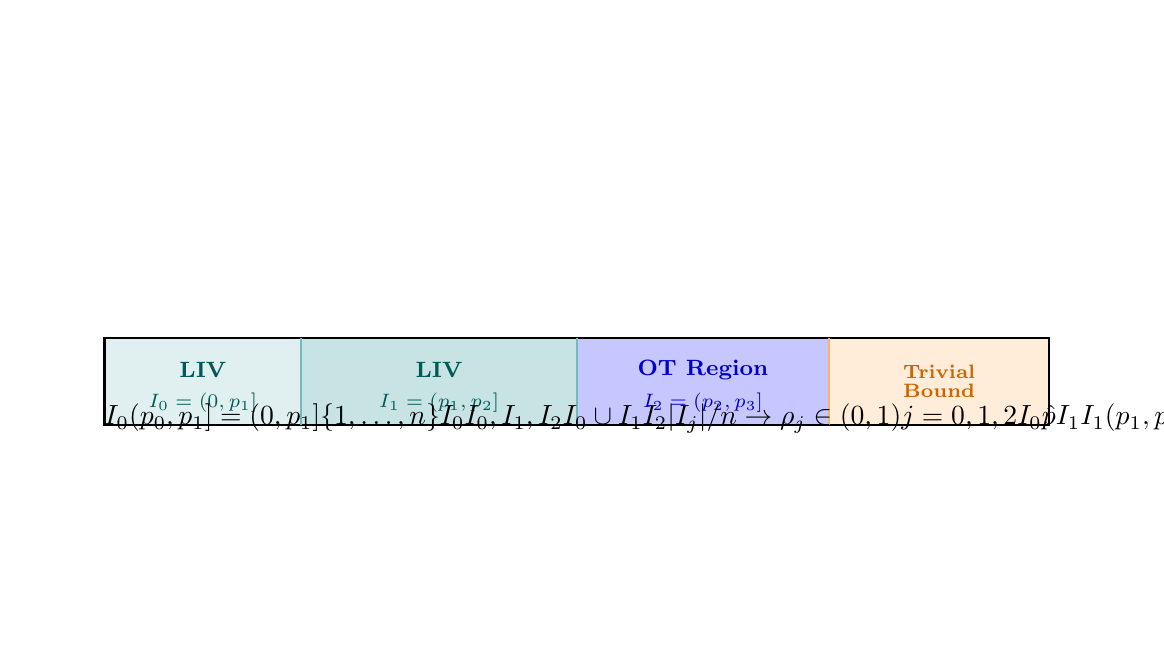
\begin{tikzpicture}[scale=1.0, font=\small]
  %% --- Layout (K=3 propensity levels for illustration) ---
  \def\W{12.0}    % full width (U = 1)
  \def\SH{1.10}   % main strip height
  \def\pA{2.5}    % p_1
  \def\pB{6.0}    % p_2
  \def\pC{9.2}    % p_3
  \def\qS{7.5}    % q* strictly between p_2 and p_3 (intermediate step in omega)
  % omega panel: baseline at y=2.20, levels measured upward
  \def\omY{2.20}  % omega y-baseline (omega = 0 line)
  \def\omA{1.80}  % omega height on I_0
  \def\omB{1.10}  % omega height on I_1
  \def\omC{0.65}  % omega height on (p_2, q*] subset of I_2
  \def\omD{0.35}  % omega height on (q*, p_3] subset of I_2
  \def\omE{0.16}  % omega height on trivial region I_3 (non-zero!)

  %% --- Main identification strip ---
  % I_0, I_1: LIV (omega constant on interval -> integral identifiable)
  \fill[teal!12]   (0,0)    rectangle (\pA,\SH);
  \fill[teal!22]   (\pA,0)  rectangle (\pB,\SH);
  % I_2: OT (omega has interior step at q* -> need quantile pairing)
  \fill[blue!22]   (\pB,0)  rectangle (\pC,\SH);
  % I_3: trivial bound
  \fill[orange!15] (\pC,0)  rectangle (\W,\SH);
  \draw[thick]     (0,0)    rectangle (\W,\SH);
  \draw[thick, teal!55]   (\pA,0) -- (\pA,\SH);
  \draw[thick, teal!55]   (\pB,0) -- (\pB,\SH);
  \draw[thick, orange!60] (\pC,0) -- (\pC,\SH);

  % Region labels inside strip
  \node[teal!70!black,  font=\footnotesize\bfseries] at (\pA/2,         0.70) {LIV};
  \node[teal!70!black,  font=\scriptsize]            at (\pA/2,         0.28) {$I_0=(0,p_1]$};
  \node[teal!70!black,  font=\footnotesize\bfseries] at ({(\pA+\pB)/2}, 0.70) {LIV};
  \node[teal!70!black,  font=\scriptsize]            at ({(\pA+\pB)/2}, 0.28) {$I_1=(p_1,p_2]$};
  \node[blue!80!black,  font=\footnotesize\bfseries] at ({(\pB+\pC)/2}, 0.70) {OT Region};
  \node[blue!80!black,  font=\scriptsize]            at ({(\pB+\pC)/2}, 0.28) {$I_2=(p_2,p_3]$};
  \node[orange!80!black, font=\scriptsize\bfseries, align=center]
      at ({(\pC+\W)/2}, \SH/2) {Trivial\\[-1pt]Bound};

\noindent\textit{Remark (notation).} $I_0$ denotes the latent interval $(p_0,p_1]=(0,p_1]$ in the latent-interval decomposition and a sample index set contained in $\{1,\ldots,n\}$ in sample splitting. In Theorem~\ref{thm:continuous_rate}, Corollary~\ref{cor:continuous_primitive_rate}: $I_0$ is the sample index set in the three-way partition $I_0,I_1,I_2$; $I_0\cup I_1$ supplies the training samples on which the target-evaluation expectations are conditioned, and $I_2$ supplies evaluation observations, with $|I_j|/n\to\rho_j\in(0,1)$ for $j=0,1,2$. In Corollary~\ref{cor:continuous_primitive_rate}: $I_0$ trains $\hat p$ and the derived policy and endpoint fits; conditional on this training sample, $I_1$ trains the outcome regression and treated boundary-law learner. $I_1$ denotes $(p_1,p_2]$ in the latent-resistance decomposition and a subset of $\{1,\ldots,n\}$ in the estimation procedures. In Lemma~\ref{lem:orthogonality_discrete}, Theorem~\ref{thm:dml_normality}: $I_1$ is the auxiliary sample index set in the random disjoint partition into $I_1$ and $I_2$, each of size $n/2$; the propensity and remaining score nuisances are fitted on $I_1$, with level recovery using the covariates in $I_2$. In Theorem~\ref{thm:continuous_rate}, Corollary~\ref{cor:continuous_primitive_rate}: $I_1$ is the nuisance sample index set in the three-way partition into $I_0,I_1,I_2$, with $|I_1|/n\to\rho_1\in(0,1)$; $I_0\cup I_1$ supplies the training samples and $I_2$ supplies target evaluation. In Corollary~\ref{cor:continuous_primitive_rate}: Conditional on the propensity fit from $I_0$, $I_1$ is used to fit $\hat g_1$ and the treated boundary law. $I_2$ denotes the latent interval $(p_2,p_3]$ in the interval decomposition and the main evaluation sample index set in estimation. In Theorem~\ref{thm:dml_normality}: $I_2\subseteq\{1,\ldots,n\}$ is the main estimation index set, disjoint from $I_1$, with $I_1\cup I_2=\{1,\ldots,n\}$ and $|I_2|=n/2$; its covariates are also used to recover the finite level sets before evaluation scores are averaged over it. In Theorem~\ref{thm:continuous_rate}, Corollary~\ref{cor:continuous_primitive_rate}: $I_2\subseteq\{1,\ldots,n\}$ is the evaluation index set in the disjoint partition $I_0,I_1,I_2$, with $|I_j|/n\to\rho_j\in(0,1)$ for $j=0,1,2$; it evaluates the target using nuisances fitted on $I_0$ and $I_1$.


  %% --- Identified-measure markers at propensity levels ---
  % p_1
  \draw[blue!55, thick] (\pA,\SH) -- (\pA,{\SH+0.30});
  \filldraw[fill=white, draw=blue!65, thick] (\pA,{\SH+0.30}) circle (3pt);
  \node[above, font=\scriptsize, blue!70!black, align=center] at (\pA,{\SH+0.30})
      {$p_1$\\[-1pt]{\tiny identified}};
  % p_2
  \draw[blue!55, thick] (\pB,\SH) -- (\pB,{\SH+0.30});
  \filldraw[fill=white, draw=blue!65, thick] (\pB,{\SH+0.30}) circle (3pt);
  \node[above, font=\scriptsize, blue!70!black, align=center] at (\pB,{\SH+0.30})
      {$p_2$\\[-1pt]{\tiny identified}};
  % p_3
  \draw[blue!55, thick] (\pC,\SH) -- (\pC,{\SH+0.30});
  \filldraw[fill=white, draw=blue!65, thick] (\pC,{\SH+0.30}) circle (3pt);
  \node[above, font=\scriptsize, blue!70!black, align=center] at (\pC,{\SH+0.30})
      {$p_3$\\[-1pt]{\tiny identified}};

  %% --- U axis ---
  \draw[->,thick] (-0.3,-0.50) -- (\W+0.6,-0.50) node[right]{$U$};
  \draw (0,   -0.38) -- (0,   -0.60); \node[below,font=\scriptsize] at (0,   -0.60) {$0$};
  \draw (\pA, -0.38) -- (\pA, -0.60); \node[below,font=\scriptsize] at (\pA, -0.60) {$p_1$};
  \draw (\pB, -0.38) -- (\pB, -0.60); \node[below,font=\scriptsize] at (\pB, -0.60) {$p_2$};
  % q* tick (shorter, different style to distinguish from propensity levels)
  \draw[gray!65] (\qS,-0.38) -- (\qS,-0.55);
  \node[below,font=\scriptsize,gray!75] at (\qS,-0.55) {$q^*$};
  \draw (\pC, -0.38) -- (\pC, -0.60); \node[below,font=\scriptsize] at (\pC, -0.60) {$p_3$};
  \draw (\W,  -0.38) -- (\W,  -0.60); \node[below,font=\scriptsize] at (\W,  -0.60) {$1$};

  %% --- Dashed vertical guides through all panels ---
  \draw[gray!40,dashed,thin] (\pA,-0.60) -- (\pA,{\omY+\omA+0.25});
  \draw[gray!40,dashed,thin] (\pB,-0.60) -- (\pB,{\omY+\omA+0.25});
  % q* guide (dotted, lighter -- not a propensity level)
  \draw[gray!35,dotted,thin] (\qS,-0.55) -- (\qS,{\omY+\omA+0.25});
  \draw[gray!40,dashed,thin] (\pC,-0.60) -- (\pC,{\omY+\omA+0.25});

  %% --- Omega piecewise-constant panel ---
  \draw[->,thick] (-0.3,\omY) -- (-0.3,{\omY+\omA+0.55})
      node[above,font=\scriptsize]{$\omega(u)$};
  \draw[gray!30,thin] (0,\omY) -- (\W,\omY);       % zero baseline
  \node[left,font=\scriptsize,gray] at (-0.3,\omY) {$0$};

  % y-axis tick marks
  \draw[gray!45] (-0.42,{\omY+\omA}) -- (-0.18,{\omY+\omA});
  \node[left,font=\scriptsize,gray!60] at (-0.42,{\omY+\omA}) {$\omega_0$};
  \draw[gray!45] (-0.42,{\omY+\omB}) -- (-0.18,{\omY+\omB});
  \node[left,font=\scriptsize,gray!60] at (-0.42,{\omY+\omB}) {$\omega_1$};
  \draw[gray!35] (-0.42,{\omY+\omC}) -- (-0.18,{\omY+\omC});  % unlabeled
  \draw[gray!35] (-0.42,{\omY+\omD}) -- (-0.18,{\omY+\omD});  % unlabeled
  \draw[gray!45] (-0.42,{\omY+\omE}) -- (-0.18,{\omY+\omE});
  \node[left,font=\scriptsize,gray!60] at (-0.42,{\omY+\omE}) {$\omega_4$};

  % piecewise-constant step function (non-increasing, with intermediate step at q*)
  \draw[thick, violet!80!black]
      (0,    {\omY+\omA}) -- (\pA, {\omY+\omA})   % constant on I_0
      -- (\pA, {\omY+\omB})                         % drop at p_1
      -- (\pB, {\omY+\omB})                         % constant on I_1
      -- (\pB, {\omY+\omC})                         % drop at p_2
      -- (\qS, {\omY+\omC})                         % constant on (p_2, q*]
      -- (\qS, {\omY+\omD})                         % drop at q* (strictly between p_2 and p_3!)
      -- (\pC, {\omY+\omD})                         % constant on (q*, p_3]
      -- (\pC, {\omY+\omE})                         % drop at p_3 (to non-zero level!)
      -- (\W,  {\omY+\omE});                        % non-zero weight in trivial region!

  %% --- Connecting arrows (strip to bound labels) ---
  \draw[->,dashed,teal!50]    (\pA/2,         0) -- (\pA/2,         -1.00);
  \draw[->,dashed,teal!50]    ({(\pA+\pB)/2}, 0) -- ({(\pA+\pB)/2}, -1.00);
  \draw[->,dashed,blue!40]    ({(\pB+\pC)/2}, 0) -- ({(\pB+\pC)/2}, -1.00);
  \draw[->,dashed,orange!55]  ({(\pC+\W)/2},  0) -- ({(\pC+\W)/2},  -1.00);

  %% --- Brief per-region bound labels ---
  % LIV regions: omega constant -> integral is directly identifiable mean
  \node[teal!70!black, font=\scriptsize, align=center]
      at (\pA/2,         -1.38) {direct\\mean};
  \node[teal!70!black, font=\scriptsize, align=center]
      at ({(\pA+\pB)/2}, -1.38) {direct\\mean};
  % OT region: omega has interior step -> quantile pairing needed
  \node[blue!75!black, font=\scriptsize, align=center]
      at ({(\pB+\pC)/2}, -1.38) {quantile\\pairing};
  \node[orange!80!black, font=\scriptsize, align=center]
      at ({(\pC+\W)/2},  -1.38) {assign $y_{\min}$};

  % plus signs between labels
  \node[font=\footnotesize] at ({(\pA/2+(\pA+\pB)/2)/2},        -1.38) {$+$};
  \node[font=\footnotesize] at ({((\pA+\pB)/2+(\pB+\pC)/2)/2},  -1.38) {$+$};
  \node[font=\footnotesize] at ({((\pB+\pC)/2+(\pC+\W)/2)/2},   -1.38) {$+$};

  %% --- Annotation explaining LIV vs OT distinction in omega panel ---
  % Arrow at p_1 drop: "drop at p_k -> LIV"
  \draw[->,gray!60,thin] (\pA+0.15,{\omY+(\omA+\omB)/2}) -- (\pA+1.2,{\omY+(\omA+\omB)/2});
  \node[right,font=\tiny,teal!65!black] at (\pA+1.2,{\omY+(\omA+\omB)/2})
      {drop at $p_k$ $\Rightarrow$ \textbf{LIV}};
  % Arrow at q* drop: "drop at q* -> OT"
  \draw[->,gray!60,thin] (\qS+0.15,{\omY+(\omC+\omD)/2}) -- (\qS+1.0,{\omY+(\omC+\omD)/2});
  \node[right,font=\tiny,blue!70!black] at (\qS+1.0,{\omY+(\omC+\omD)/2})
      {drop at $q^*$ $\Rightarrow$ \textbf{OT}};

\noindent\textit{Remark (notation).} $p_k(x)$ denotes an ordered population baseline propensity level, with $p_k(x)=p(z,x)$ for $z\in S_k$ and $k=1,\ldots,K$, while $p_0(x)=0$ and $p_{K+1}(x)=1$ are structural integration boundaries; $K$ and the level sets $S_k$ are invariant in $x$.


  %% --- Global sharp lower bound formula ---
  \node[align=center, font=\footnotesize] at ({\W/2}, -2.30) {
    $
    \underline{\theta}_{\omega,1}
    \;=\; \sum_{i=0}^{K-1}(p_{i+1}-p_i)
      \int_0^1 Q_{Y,i}(t)\,Q_{\omega,i}(1-t)\,\mathrm{d}t
    \;+\; \int_{p_K}^{1}\!\bigl(y_{\min}[\omega]_+\!+y_{\max}[\omega]_-\bigr)\mathrm{d}u$
  };

\end{tikzpicture}
\caption{Decomposition of the latent-resistance interval $[0,1]$ for the sharp lower bound in \cref{thm:discrete_lower_bound} with $K=3$ propensity levels. In the \textbf{\color{teal!65}LIV regions} $I_0$ and $I_1$, the weight $\omega(u)$ is constant within each interval, so the contribution is an identified conditional mean. In the \textbf{\color{blue!65}OT region} $I_2$, $\omega(u)$ changes inside the interval, so the sharp bound depends on the coupling between $Y(1)$ and $\omega(U)$ and is attained by countermonotone quantile pairing. In the \textbf{\color{orange!65}trivial region} $I_3$, $Y(1)$ is unobserved, so the lower bound assigns the worst feasible outcome value pointwise. The top panel shows the piecewise-constant $\omega(u)$; the bottom row gives the bound contribution per region.}
\label{fig:decomposition}
\end{figure}

By \cref{thm:discrete_lower_bound}, the width of the identified interval is
\begin{equation*}
\begin{aligned}
\overline{\theta }_{\omega ,1} -\underline{\theta }_{\omega ,1}
& =\sum _{i=0}^{K-1} (p_{i+1} -p_{i} )\int _{0}^{1}( Q_{Y,i} (t)-Q_{Y,i}( 1-t)) Q_{\omega ,i} (t) \mathrm{d} t \\
& \quad + ( y_{\max} -y_{\min})\int _{p_{K}}^{1} |\omega (u)| \mathrm{d} u,
\end{aligned}
\end{equation*}
which depends on the range of the propensity function and on the distributions $\mu_{1,i}$. If $p_K$ is close to $1$ and the support of each $\mu_{1,i}$ is small, the width is also small. In particular, if each $Q_{Y,i}$ is constant and $p_K = 1$, then $\theta_{\omega,1}$ is point-identified from the data.

\begin{remark}[Decomposition into 1D marginal constraints and \citet{marx2024sharp}] \label{rem:marx-open}
\citet{marx2024sharp} raises the open question of characterizing the distribution of treatment effects for the complier group. Although \cref{prop:sharpness} states sharpness at the joint level of $(Y(0), Y(1), U, X)$, the CCOT constraints defining $\Gamma(\mathbb{P}_{obs})$ reduce to independent one-dimensional marginal constraints on the conditional kernels $\pi_w(\diff y \mid u, x)$, so once these marginals are pinned down the remaining freedom lies entirely in the coupling between $Y(1)$ and $Y(0)$ given $(U, X)$. In the binary-instrument, no-covariate setting with $p_1 < p_2$, the complier interval is $I_c=(p_1,p_2]$ and (\ref{eq:y_identified_measure}) identifies the treated-outcome distribution for compliers as $\mu_{1,1}$; differencing the untreated component, which is nonincreasing in $p$, identifies
\[
\mu_{0,1}(\diff y)
:=
\frac{\mathbb{P}_{obs}(\diff y, W=0 \mid p(Z)=p_1)-\mathbb{P}_{obs}(\diff y, W=0 \mid p(Z)=p_2)}{p_2-p_1}.
\]
The identified set for the complier treatment-effect distribution is therefore exactly $\mathcal I_{\Delta,c} = \{(y_1-y_0)_{\#}\gamma : \gamma \in \Pi(\mu_{1,1},\mu_{0,1})\}$, so Marx's question becomes: once the identified complier marginals are fixed, characterize all pushforwards of their couplings under $(y_1,y_0)\mapsto y_1-y_0$. Characterizing $\mathcal I_{\Delta,c}$ therefore reduces to determining the treatment-effect distributions generated by these couplings.
\end{remark}

\subsubsection{General Instrument Setting}\label{subsubsec:continuous_iv}
We now consider a general instrument setting under a single regularity condition on the instrument domain and the propensity score. This framework nests the finite discrete case (each component a singleton), the connected continuous case studied in the local instrumental variables (LIV) literature \citep{heckman1999local}, and mixtures of the two.

\begin{assumption}[Finite-Component Propensity Continuity]\label{asp:continuity_p}
    The instrument domain $\mathcal{Z}$ has finitely many connected components. For almost every $x \in \mathcal{X}$, the conditional propensity score function $z \mapsto p(z,x) = \mathbb{P}(W=1 \mid Z=z, X=x)$ is continuous on each connected component.
\end{assumption}

\noindent\textit{Remark.} The continuity condition holds for $\mathbb P_X$-almost every $x\in\mathcal X$.


Under the standing compactness of $\mathcal Z$ and \cref{asp:continuity_p}, the image of each connected component under $p(\cdot)$ is a closed interval (possibly a singleton if $p$ is constant on the component or if the component is a single point). Merging overlaps and ordering from left to right, the range of the propensity score admits a maximal-interval decomposition
\begin{equation}\label{eq:range_decomposition}
    p(\mathcal{Z}) \;=\; \bigcup_{k=1}^{K}\bigl[\underline{p}_k,\overline{p}_k\bigr], \qquad 0 \leqslant \underline{p}_1 \leqslant \overline{p}_1 < \underline{p}_2 \leqslant \overline{p}_2 < \cdots < \underline{p}_K \leqslant \overline{p}_K \leqslant 1,
\end{equation}
where we explicitly allow degenerate intervals $\underline{p}_k = \overline{p}_k$ corresponding to isolated propensity values, as in the finite discrete case. Adopting the boundary conventions $\overline{p}_0 := 0$ and $\underline{p}_{K+1} := 1$, this decomposition partitions the unit interval of the latent variable $U$ into three types of regions: the LIV intervals $L_k := [\underline{p}_k,\overline{p}_k]$ for $k=1,\dots,K$, the OT gaps $G_k := (\overline{p}_k, \underline{p}_{k+1})$ for $k=0,\dots,K-1$, and the trivial tail $(\overline{p}_K,1]$.

\noindent\textit{Remark (notation).} $\underline p_k$ denotes the left endpoint of the $k$-th maximal closed interval in the propensity range ordered from left to right, allowing singleton intervals. In Theorem~\ref{thm:continuous_lower_bound}: The endpoints are indexed by $k=1,\ldots,K$ in $p(\mathcal Z)=\bigcup_{k=1}^K[\underline p_k,\overline p_k]$, with the additional boundary convention $\underline p_{K+1}=1$. In Theorem~\ref{thm:covariate_continuous_lower_bound}: For almost every $x$, the endpoint is $\underline p_k(x)$, indexed by $k=1,\ldots,K_x$ in the conditional range $p(\mathcal Z,x)$, with $\underline p_{K_x+1}(x)=1$; both endpoints and the component count may vary with $x$. $\overline p_k$ denotes the right endpoint of the $k$-th maximal closed interval in the propensity range ordered from left to right, allowing singleton intervals and using zero as the auxiliary initial endpoint. In Theorem~\ref{thm:continuous_lower_bound}: The endpoints are indexed by $k=1,\ldots,K$ in $p(\mathcal Z)=\bigcup_{k=1}^K[\underline p_k,\overline p_k]$, with $\overline p_0=0$. In Theorem~\ref{thm:covariate_continuous_lower_bound}: For almost every $x$, the endpoint is $\overline p_k(x)$, indexed by $k=1,\ldots,K_x$ in $p(\mathcal Z,x)$, with $\overline p_0(x)=0$; endpoints and the component count may vary with $x$. In Proposition~\ref{prop:discrete_reduction}, Proposition~\ref{prop:J_specialization}: Each conditional range component is a singleton: $\underline p_k(x)=\overline p_k(x)=p_k(x)$ for $k=1,\ldots,K$, with the structural initial endpoint $p_0(x)=\overline p_0(x)=0$. $L_k$ denotes the $k$-th closed maximal interval of the propensity range, ordered from left to right, including singleton intervals. In Theorem~\ref{thm:continuous_lower_bound}: $L_k=[\underline p_k,\overline p_k]$ for $k=1,\ldots,K$; singleton intervals contribute a Lebesgue-null integral. In Theorem~\ref{thm:covariate_continuous_lower_bound}: For almost every $x$, $L_k(x)=[\underline p_k(x),\overline p_k(x)]$ for $k=1,\ldots,K_x$; the intervals are those of $p(\mathcal Z,x)$ and may be singletons. $G_k$ denotes the open interval between consecutive ordered propensity-range components, with the initial gap starting at zero and with the final unconstrained tail excluded from the gap indices. In Theorem~\ref{thm:continuous_lower_bound}: $G_k=(\overline p_k,\underline p_{k+1})$ for $k=0,\ldots,K-1$, with $\overline p_0=0$; empty gaps are omitted from gap-specific definitions and contribute zero. In Theorem~\ref{thm:covariate_continuous_lower_bound}: $G_k(x)=(\overline p_k(x),\underline p_{k+1}(x))$ for $k=0,\ldots,K_x-1$ and almost every $x$, with $\overline p_0(x)=0$; empty conditional gaps contribute zero. In Proposition~\ref{prop:discrete_reduction}, Proposition~\ref{prop:J_specialization}: The propensity-range components are singletons, so $G_k(x)=(p_k(x),p_{k+1}(x))$ for $k=0,\ldots,K-1$, with $p_0(x)=0$; the interval beyond $p_K(x)$ is the separate trivial tail. $\underline p(x)=\inf_{z\in\mathcal Z}p(z,x)$ is the population lower propensity endpoint at covariate value $x$, with values in $[0,1]$ and with zero allowed. In Proposition~\ref{prop:continuous_reduction}, Theorem~\ref{thm:continuous_rate}, Corollary~\ref{cor:continuous_primitive_rate}: $\underline p(x)$ is the lower endpoint of the connected conditional support $[\underline p(x),\overline p(x)]$ of $P\mid X=x$. $\overline p(x)=\sup_{z\in\mathcal Z}p(z,x)$ is the population upper propensity endpoint at covariate value $x$, with values in $[0,1]$. In Proposition~\ref{prop:continuous_reduction}, Theorem~\ref{thm:continuous_rate}, Corollary~\ref{cor:continuous_primitive_rate}: $\overline p(x)$ is the upper endpoint of the connected conditional support $[\underline p(x),\overline p(x)]$ of $P\mid X=x$. $\bar p_2(z)$ is the sample-dependent average of the clipped first-stage fit $\hat p(z,\cdot)$ trained on $I_1$ over the covariates indexed by $I_2$; conditional on $I_1$ it remains an empirical average over evaluation covariates, rather than the population marginal mean.


The CCOT problem for the treated ($W=1$) component becomes
\begin{equation}\label{eq:ot_formulation_continuous}
    \begin{split}
        \min_{\pi_1}\quad &  \mathbb{E}_{\pi_1}[Y(1)\omega(U)]  \\
        \text{subject to}  \quad &  \int_0^{p} \pi_{1}(\mathrm{d}y \mid u) \mathrm{d}u = H_1(p,\mathrm{d}y), \ \forall p \in p(\mathcal{Z}), \\
        & \pi_1(\mathrm{d}u) = \mathrm{d}u.
    \end{split}
\end{equation}
Following the same strategy as in \cref{subsubsec:discrete_iv}, we rewrite (\ref{eq:ot_formulation_continuous}) into a manifestly separable form across the three region types. The objective splits additively as
\begin{align*}
\mathbb{E}_{\pi_1}[Y(1)\omega(U)]
&= \sum_{k=0}^{K-1}\int_{G_k}\!\int_{\mathcal{Y}} y\,\omega(u)\,\pi_1(\mathrm{d}y\mid u)\,\mathrm{d}u
+ \sum_{k=1}^{K}\int_{L_k}\!\int_{\mathcal{Y}} y\,\omega(u)\,\pi_1(\mathrm{d}y\mid u)\,\mathrm{d}u \\
&\quad\quad+ \int_{\overline{p}_K}^{1}\!\int_{\mathcal{Y}} y\,\omega(u)\,\pi_1(\mathrm{d}y\mid u)\,\mathrm{d}u.
\end{align*}
On each gap $G_k$, the same telescoping argument that produced (\ref{eq:y_identified_measure})---differencing the observational constraint in (\ref{eq:ot_formulation_continuous}) at $p=\overline{p}_k$ and $p=\underline{p}_{k+1}$---fixes the marginal of $Y(1)$ on $G_k$ to be
\begin{equation}\label{eq:gap_identified_measure}
    \mu_{1,k}(\mathrm{d}y) \;:=\; \frac{H_1(\underline{p}_{k+1},\mathrm{d}y)-H_1(\overline{p}_k,\mathrm{d}y)}{\underline{p}_{k+1}-\overline{p}_k}, \qquad k:\ \overline p_k<\underline p_{k+1},
\end{equation}
where $H_1(0,\cdot)=0$ by definition. Thus the $k=0$ formula applies when $\underline p_1>0$; when $\underline p_1=0$, $G_0$ is empty and has zero contribution. More generally, empty gaps are omitted from all gap-specific definitions and sums below. Let $g_1^{\mathrm c}(p)\coloneqq\int_{\mathcal Y}y\,H_1(p,\mathrm{d}y)$, and fix the countable measure-determining class $\mathcal A:=\{\mathcal Y\cap(-\infty,r]:r\in\mathbb Q\}\cup\{\mathcal Y\}$. On each non-degenerate LIV interval $L_k$, the constraint in (\ref{eq:ot_formulation_continuous}) holds for every $p\in[\underline{p}_k,\overline{p}_k]$. For each $A\in\mathcal A$, the scalar map $p\mapsto H_1(p,A)$ is absolutely continuous on $L_k$ and the ordinary fundamental theorem of calculus gives
\begin{equation}\label{eq:liv_identity}
\pi_1(A\mid u) \;=\; \frac{\partial}{\partial p}\bigg|_{p=u}H_1(p,A),
\qquad A\in\mathcal A,\quad u\in L_k\ \text{a.e.}
\end{equation}
Countability of $\mathcal A$ gives one common null set, so (\ref{eq:liv_identity}) identifies $\pi_1(\cdot\mid u)$ almost everywhere on $L_k$. Applying the same scalar argument to the bounded function $y$ gives $\partial_u g_1^{\mathrm c}(u)=\int_{\mathcal Y}y\,\pi_1(\mathrm dy\mid u)$ almost everywhere. The trivial tail $(\overline{p}_K,1]$ carries no constraint. Because cumulative sums of the gap marginals plus integration of the identified LIV kernels recover the original constraint at every $p\in p(\mathcal{Z})$, this transformation is invertible and the two constraint systems are equivalent. Each rewritten constraint involves $\pi_1$ only on its own region and the objective is additively separable, so the global problem decomposes into three types of subproblems, one for each region type.

\noindent\textit{Remark (notation).} $\mu_{1,k}$ is the identified marginal law $\mathcal L(Y(1)\mid U\in G_k)$ on each nonempty gap $G_k$, $k\in\{0,\ldots,K-1\}$, obtained from the canonical treated submeasures, including the structural zero submeasure at the initial boundary. $g_1^{\mathrm c}(p,x)=\int_{\mathcal Y}y\,H_{1,x}(p,\mathrm dy)$ uses the canonical population observed submeasure on the conditional propensity support, including its endpoints; it is absolutely continuous on each non-degenerate LIV interval, and its derivatives mean intervalwise Lebesgue-a.e. derivatives. In Theorem~\ref{thm:continuous_lower_bound}: With no covariates, $g_1^{\mathrm c}(p)=\int_{\mathcal Y}y\,H_1(p,\mathrm dy)$, and derivatives are taken on the non-degenerate intervals $L_k$. In Proposition~\ref{prop:continuous_reduction}, Theorem~\ref{thm:continuous_rate}: $g_1=g_1^{\mathrm c}$ on the connected conditional support $[\underline p(x),\overline p(x)]$. $g_1=g_1^{\mathrm c}$ denotes the canonical population treated regression obtained by integrating $y$ against the canonical observed treated submeasure, identified on the conditional propensity support including its endpoints, with intervalwise Lebesgue-a.e. derivatives on non-degenerate LIV intervals. In Theorem~\ref{thm:continuous_lower_bound}: With no covariates, $g_1(u)=\int_{\mathcal Y}y\,H_1(u,\mathrm dy)$; derivatives are taken separately on the non-degenerate intervals $L_k$. In Proposition~\ref{prop:continuous_reduction}, Theorem~\ref{thm:continuous_rate}, Corollary~\ref{cor:continuous_primitive_rate}: The identified conditional support is $[\underline p(x),\overline p(x)]$, and target evaluations use $q^{\mathrm{tr}}(Z,X)$ and $P$ within this support.


\begin{enumerate}
    \item \textbf{The OT gaps} $G_k$, $k=0,\dots,K-1$: the $Y(1)$-marginal is fixed to $\mu_{1,k}$ of (\ref{eq:gap_identified_measure}) and the $U$-marginal is $\text{Unif}(G_k)$, so the contribution of $G_k$ is a standard 1D OT problem, solved by \cref{thm:1d_ot}. Empty gaps contribute zero.
    \item \textbf{The LIV intervals} $L_k$, $k=1,\dots,K$: for non-degenerate $L_k$, the LIV identity (\ref{eq:liv_identity}) point-identifies $\mathbb{E}[Y(1)\mid U=u]=\partial_u g_1^{\mathrm c}(u)$ for a.e.\ $u \in L_k$, so the contribution is uniquely determined. Degenerate $L_k$ contribute a Lebesgue-null integral and drop out.
    \item \textbf{The trivial tail} $(\overline{p}_K, 1]$: $Y(1)$ is never observed and the data impose no constraint, so the minimization over the compact outcome domain assigns all mass to $y_{\min}$ where $\omega(u) \geqslant 0$ and to $y_{\max}$ where $\omega(u) < 0$.
\end{enumerate}

Combining the solutions across these regions yields the closed-form sharp bounds for the general instrument setting, which are illustrated in \cref{fig:continuous_decomposition} of \supplocation.

\begin{theorem}[General Closed-Form Sharp Bounds]\label{thm:continuous_lower_bound}
    Suppose \cref{asp:structure}, \cref{asp:target_weight}, and \cref{asp:continuity_p} hold, and $X$ is almost surely constant. Let $p(\mathcal{Z}) = \bigcup_{k=1}^{K}[\underline{p}_k, \overline{p}_k]$ be the maximal-interval decomposition in (\ref{eq:range_decomposition}). For each nonempty gap $G_k$, let $Q_{Y,k}(t)$ be the quantile function of $\mu_{1,k}$ defined in (\ref{eq:gap_identified_measure}), and $Q_{\omega,k}(t)$ the quantile function of $\omega(U)$ for $U \sim \text{Unif}(G_k)$. In the displayed sums, a term indexed by an empty gap is defined to be zero. The sharp lower bound for the $W=1$ component of the target parameter is given by
    \begin{equation}\label{eq:continuous_lower_bound}
        \begin{split}
            \underline{\theta}_{\omega,1}\ =\
            & \underbrace{\sum_{k=0}^{K-1}(\underline{p}_{k+1}-\overline{p}_k)\int_0^1 Q_{Y,k}(t)\,Q_{\omega,k}(1-t)\,\mathrm{d}t}_{\text{OT Bound on the Gaps}} + \underbrace{\sum_{k=1}^{K}\int_{\underline{p}_k}^{\overline{p}_k}\frac{\diff}{\diff u}g_1^{\mathrm c}(u)\,\omega(u)\,\mathrm{d}u}_{\text{Point-Identified LIV on the Intervals}} \\
            & \quad\quad + \underbrace{\int_{\overline{p}_K}^{1}\Big(y_{\min}\max\{0,\omega(u)\} + y_{\max}\min\{0,\omega(u)\}\Big)\mathrm{d}u}_{\text{Trivial Lower Bound on the Tail}}.
        \end{split}
    \end{equation}
    Similarly, the sharp upper bound is given by replacing $Q_{\omega,k}(1-t)$ with $Q_{\omega,k}(t)$ in the OT term and swapping $y_{\min}$ and $y_{\max}$ in the trivial tail term.
    % \begin{equation*}
    %     \begin{split}
    %         \overline{\theta}_{\omega,1}\ =\
    %         & \sum_{k=0}^{K-1}(\underline{p}_{k+1}-\overline{p}_k)\int_0^1 Q_{Y,k}(t)\,Q_{\omega,k}(t)\,\mathrm{d}t \ + \ \sum_{k=1}^{K}\int_{\underline{p}_k}^{\overline{p}_k}\left(\frac{\diff}{\diff u}\mathbb{E}_{obs}[YW \mid p(Z)=u]\right)\omega(u)\,\mathrm{d}u \\
    %         & \quad\quad + \int_{\overline{p}_K}^{1}\Big(y_{\max}\max\{0,\omega(u)\} + y_{\min}\min\{0,\omega(u)\}\Big)\mathrm{d}u.
    %     \end{split}
    % \end{equation*}
\end{theorem}

\noindent\textit{Remark.} The partition assertion means $\int_{[0,1]\setminus\left(\bigcup_{k=1}^{K}L_k\,\cup\,\bigcup_{k=0}^{K-1}G_k\,\cup\,(\overline p_K,1]\right)}\mathrm du=0$. For each probability law $\mu$ used here, $Q_\mu(t)=\inf\{a\in\mathbb R:\mu(( -\infty,a])\geqslant t\}$ for $t\in(0,1)$, with the displayed quantile integrals interpreted as Lebesgue integrals over $(0,1)$.

\noindent\textit{Remark (notation).} $Q_{Y,k}$ is the quantile function of $\mu_{1,k}$ for $t\in(0,1)$ and $k\in\{0,\ldots,K-1\}$ such that $\overline p_k<\underline p_{k+1}$; an empty gap has zero contribution and requires no quantile function. $Q_{\omega,k}$ is the quantile function of the law of $\omega(U)$ under $U\sim\mathrm{Unif}(G_k)$, defined for $t\in(0,1)$ and $k\in\{0,\ldots,K-1\}$ such that $\overline p_k<\underline p_{k+1}$; an empty gap has zero contribution and requires no quantile function.


The proof combines the subtraction-of-constraints decomposition from \cref{thm:discrete_lower_bound} (applied region-by-region to identify $\mu_{1,k}$ on each gap) with the LIV-derivative argument on each non-degenerate interval $L_k$, followed by the 1D OT coupling of \cref{thm:1d_ot}. We defer the formal proof to that of \cref{thm:covariate_continuous_lower_bound} in \cref{sec:cov_proof}, which restates the result in the unified form of the covariate subsection below. \cref{thm:continuous_lower_bound} subsumes both classical settings as limit cases. When every LIV interval is degenerate ($\underline{p}_k = \overline{p}_k$ for all $k$), the LIV sum vanishes identically, each $\mu_{1,k}$ coincides with the discrete complier distribution in (\ref{eq:y_identified_measure}), and (\ref{eq:continuous_lower_bound}) reduces exactly to \cref{thm:discrete_lower_bound}. Conversely, when $K=1$ with $\underline{p}_1 < \overline{p}_1$, the gap sum contains a single OT term on $(0,\underline{p}_1)$, the LIV sum contributes a single integral on $[\underline{p}_1,\overline{p}_1]$, and we recover the connected-continuous case; in particular, we match the identification results of \citet{heckman1999local} when additionally $\underline{p}_1 = 0$ and $\overline{p}_1 = 1$, so the propensity score has full support with no gaps. The width of the identified interval depends on the gap widths, the identified gap distributions $\mu_{1,k}$, and the tail beyond $\overline{p}_K$:
\begin{align*}
    \overline{\theta}_{\omega,1} - \underline{\theta}_{\omega,1}
    &= \sum_{k=0}^{K-1}(\underline{p}_{k+1}-\overline{p}_k)\int_0^1\Big(Q_{Y,k}(t) - Q_{Y,k}(1-t)\Big)Q_{\omega,k}(t)\,\mathrm{d}t \\
    &\quad + (y_{\max}-y_{\min})\int_{\overline{p}_K}^{1}|\omega(u)|\,\mathrm{d}u.
\end{align*}



\subsection{Closed-Form Bounds with Covariates}\label{subsec:cf_cov}

Generalizing the previous results to covariates is mathematically straightforward. Because \cref{asp:structure} imposes $Z \indep (Y(w), U) \mid X$, the global CCOT problem disintegrates into a family of conditional one-dimensional optimal transport problems indexed by $x \in \mathcal{X}$: we solve conditional on $X=x$ and aggregate the conditional bounds over the marginal distribution of $X$ by iterated expectations.

Under \cref{asp:continuity_p}, for $\mathbb{P}_{obs}$-a.e.\ $x \in \mathcal{X}$, the conditional range of the propensity score admits a maximal-interval decomposition
\begin{equation}\label{eq:range_decomposition_cov}
    p(\mathcal{Z}, x) \;=\; \bigcup_{k=1}^{K_x}[\underline{p}_k(x), \overline{p}_k(x)], \qquad 0 \leqslant \underline{p}_1(x) \leqslant \overline{p}_1(x) < \cdots < \underline{p}_{K_x}(x) \leqslant \overline{p}_{K_x}(x) \leqslant 1,
\end{equation}
with degenerate intervals $\underline{p}_k(x) = \overline{p}_k(x)$ corresponding to isolated conditional propensity values and boundary conventions $\overline{p}_0(x) := 0$ and $\underline{p}_{K_x+1}(x) := 1$. For each $x$, this partitions $[0,1]$ into the conditional LIV intervals $L_k(x) := [\underline{p}_k(x), \overline{p}_k(x)]$, the OT gaps $G_k(x) := (\overline{p}_k(x), \underline{p}_{k+1}(x))$, and the trivial tail $(\overline{p}_{K_x}(x), 1]$. The conditional gap-identified measure of $Y(1)$ on $G_k(x)$ is
\begin{equation}\label{eq:gap_identified_measure_cov}
    \mu_{1,k\mid x}(\mathrm{d}y) \;:=\; \frac{H_{1,x}(\underline{p}_{k+1}(x),\mathrm{d}y)-H_{1,x}(\overline{p}_k(x),\mathrm{d}y)}{\underline{p}_{k+1}(x)-\overline{p}_k(x)},
\end{equation}
for indices $k$ such that $\overline p_k(x)<\underline p_{k+1}(x)$; $H_{1,x}(0,\cdot)=0$ by definition. Empty conditional gaps are omitted and contribute zero. Finally, let $g_1^{\mathrm c}(p,x)\coloneqq\int_{\mathcal Y}y\,H_{1,x}(p,\mathrm{d}y)$. This canonical version is absolutely continuous in $p$ on each non-degenerate LIV interval $L_k(x)$, and every derivative below means its intervalwise Lebesgue-a.e. derivative.

\noindent\textit{Remark (notation).} For almost every $x$, $K_x$ is the finite number of closed maximal intervals, including singleton intervals, obtained by merging overlapping component images in $p(\mathcal Z,x)$; its value may depend on $x$. In Proposition~\ref{prop:continuous_reduction}: The instrument domain is connected, so $K_x=1$ and the sole conditional range interval is $[\underline p(x),\overline p(x)]$, possibly a singleton. $\mu_{1,k\mid x}$ is the population probability law of $Y(1)$ conditional on $X=x$ and $U\in G_k(x)$, defined for nonempty gaps with $k=0,\ldots,K_x-1$; empty-gap terms are omitted and contribute zero. In Proposition~\ref{prop:discrete_reduction}, Proposition~\ref{prop:J_specialization}, Lemma~\ref{lem:orthogonality_discrete}: With finite $\mathcal Z$, the conditional propensity-range intervals are singletons, $G_k(x)=(p_k(x),p_{k+1}(x))$ for $k=0,\ldots,K-1$, and $\mu_{1,k\mid x}$ is the corresponding conditional complier outcome law.


\begin{theorem}[Conditional General Bound]\label{thm:covariate_continuous_lower_bound}
    Suppose \cref{asp:structure}, \cref{asp:target_weight}, and \cref{asp:continuity_p} hold. For each nonempty conditional gap $G_k(x)$, let $Q_{Y, k \mid x}(t)$ be the quantile function of $\mu_{1,k\mid x}$ defined in (\ref{eq:gap_identified_measure_cov}), and $Q_{\omega, k \mid x}(t)$ the quantile function of $\omega(x, U)$ for $U \sim \text{Unif}(G_k(x))$. In the displayed sums, a term indexed by an empty conditional gap is defined to be zero. The sharp lower bound for the $W=1$ component of the target parameter is
    \begin{equation} \label{eq:covariate_continuous_lower_bound}
        \begin{split}
        \underline{\theta}_{\omega,1}  = \mathbb{E}_{X} \Bigg[ & \sum_{k=0}^{K_X-1}(\underline{p}_{k+1}(X)-\overline{p}_k(X))\int_0^1 Q_{Y,k\mid X}(t)\,Q_{\omega,k\mid X}(1-t)\,\mathrm{d}t \\
        & + \sum_{k=1}^{K_X}\int_{\underline{p}_k(X)}^{\overline{p}_k(X)} \frac{\diff}{\diff u}g_1^{\mathrm c}(u,X)\, \omega(X, u) \, \mathrm{d}u \\
        & + \int_{\overline{p}_{K_X}(X)}^1 \Big( y_{\min} \max\{0, \omega(X, u)\} + y_{\max} \min\{0, \omega(X, u)\} \Big) \mathrm{d}u \Bigg].
        \end{split}
    \end{equation}
    Similarly, the sharp upper bound is given by replacing $Q_{\omega,k\mid X}(1-t)$ with $Q_{\omega,k\mid X}(t)$ in the OT term and swapping $y_{\min}$ and $y_{\max}$ in the trivial tail term.
    % \begin{equation*}
    %     \begin{split}
    %     \overline{\theta}_{\omega,1}  = \mathbb{E}_{X} \Bigg[ & \sum_{k=0}^{K_X-1}(\underline{p}_{k+1}(X)-\overline{p}_k(X))\int_0^1 Q_{Y,k\mid X}(t)\,Q_{\omega,k\mid X}(t)\,\mathrm{d}t \\
    %     & + \sum_{k=1}^{K_X}\int_{\underline{p}_k(X)}^{\overline{p}_k(X)} \left( \frac{\diff }{\diff u} \mathbb{E}_{obs}[Y W \mid p(Z,X)=u, X] \right) \omega(X, u) \, \mathrm{d}u  \\
    %     & + \int_{\overline{p}_{K_X}(X)}^1 \Big( y_{\max} \max\{0, \omega(X, u)\} + y_{\min} \min\{0, \omega(X, u)\} \Big) \mathrm{d}u \Bigg].
    %     \end{split}
    % \end{equation*}

\emph{Additional condition.} For every nonempty conditional gap $G_k(x)$, extend $Q_{Y,k\mid x}$ to $[0,1]$ by $Q_{Y,k\mid x}(0):=y_{\min}$ and $Q_{Y,k\mid x}(1):=y_{\max}$.
\end{theorem}

\noindent\textit{Remark.} For every nonempty conditional gap $G_k(x)$ and $0<t<1$, $(Q_{Y,k\mid x}(t),Q_{\omega,k\mid x}(t))=(\inf\{y\in\mathbb R:\mu_{1,k\mid x}(\mathcal Y\cap(-\infty,y])\geqslant t\},\inf\{v\in\mathbb R:F_{\omega,k\mid x}(v)\geqslant t\})$. For $\mathbb P_X$-almost every $x$, the intervals $L_k(x)$, $1\leqslant k\leqslant K_x$, the gaps $G_k(x)$, $0\leqslant k<K_x$, and the tail $(\overline p_{K_x}(x),1]$ partition $[0,1]$ up to Lebesgue-null endpoints. For $0<t<1$, use the lower generalized inverses $Q_{Y,k\mid x}(t)=\inf\{y\in\mathbb R:\mu_{1,k\mid x}(\mathcal Y\cap(-\infty,y])\geqslant t\}$ and $Q_{\omega,k\mid x}(t)=\inf\{v\in\mathbb R:F_{\omega,k\mid x}(v)\geqslant t\}$. Interpret the kernel formula with any fixed jointly measurable $\mathcal Y$-valued extension of $Q_{Y,k\mid x}$ to ranks $0$ and $1$; the asserted gap marginal and attaining objective hold for every such extension.

\noindent\textit{Remark (notation).} $Q_{Y,k\mid x}$ is the population quantile function of $\mu_{1,k\mid x}$ for each nonempty conditional gap $G_k(x)$; it is required only on such gaps, and contributions from empty gaps are defined as zero. In Proposition~\ref{prop:discrete_reduction}, Proposition~\ref{prop:J_specialization}, Lemma~\ref{lem:orthogonality_discrete}: In the finite-instrument setting, the gap is the baseline interval between $p_k(x)$ and $p_{k+1}(x)$, with $k=0,\ldots,K-1$, and $\mu_{1,k\mid x}$ is its identified conditional complier outcome law. $Q_{\omega,k\mid x}$ is defined for each nonempty conditional gap $G_k(x)$, $0\leqslant k<K_x$, as the quantile function of the pushforward of $\mathrm{Unif}(G_k(x))$ by $u\mapsto\omega(x,u)$; empty-gap contributions are zero without requiring a quantile function there. In Proposition~\ref{prop:discrete_reduction}: The conditional propensity-range intervals are singletons, so the relevant gap law is $\mathrm{Unif}((p_k(x),p_{k+1}(x)))$ for $k=0,\ldots,K-1$, with $p_0(x)=0$.

The proof of \cref{thm:covariate_continuous_lower_bound} is given in \cref{sec:cov_proof}. The two limit cases stated after \cref{thm:continuous_lower_bound} carry over verbatim under $x$-conditioning: degenerate conditional LIV intervals reduce (\ref{eq:covariate_continuous_lower_bound}) to the discrete covariate bound, and $K_X = 1$ with $\underline{p}_1(X) < \overline{p}_1(X)$ recovers the standard LIV covariate bound.
